\documentclass[border=0.05cm]{standalone}
\usepackage{../../../../preamble_tikz}
\usepackage{../../../../preamble_math}

\def\sepArrow{0.56}
\def\sepArrowDouble{0.615}
\def\sepx{0.5}

\begin{document}
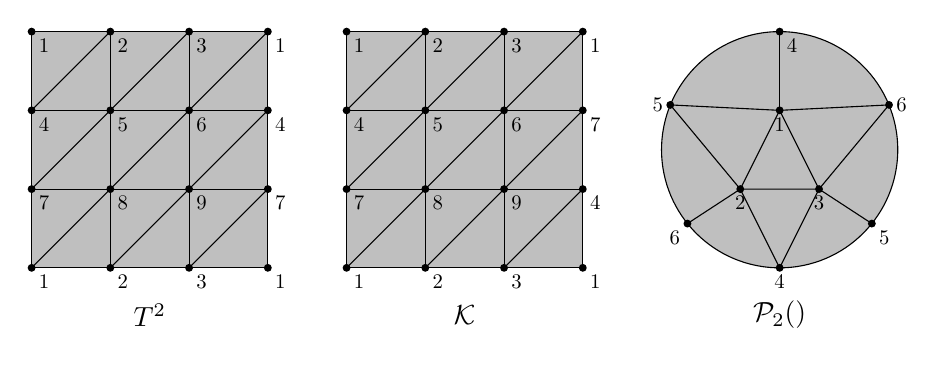
\begin{tikzpicture}


  %%% TORUS
  % grid
  \filldraw[fill=lightgray] (0,0) grid (3,3) rectangle (0,0);
  \fill (0,0) circle (0.05cm) node[anchor=north west,scale=0.75]{1};
  \fill (0,1) circle (0.05cm) node[anchor=north west,scale=0.75]{7};
  \fill (0,2) circle (0.05cm) node[anchor=north west,scale=0.75]{4};
  \fill (0,3) circle (0.05cm) node[anchor=north west,scale=0.75]{1};
  \fill (1,0) circle (0.05cm) node[anchor=north west,scale=0.75]{2};
  \fill (1,1) circle (0.05cm) node[anchor=north west,scale=0.75]{8};
  \fill (1,2) circle (0.05cm) node[anchor=north west,scale=0.75]{5};
  \fill (1,3) circle (0.05cm) node[anchor=north west,scale=0.75]{2};
  \fill (2,0) circle (0.05cm) node[anchor=north west,scale=0.75]{3};
  \fill (2,1) circle (0.05cm) node[anchor=north west,scale=0.75]{9};
  \fill (2,2) circle (0.05cm) node[anchor=north west,scale=0.75]{6};
  \fill (2,3) circle (0.05cm) node[anchor=north west,scale=0.75]{3};
  \fill (3,0) circle (0.05cm) node[anchor=north west,scale=0.75]{1};
  \fill (3,1) circle (0.05cm) node[anchor=north west,scale=0.75]{7};
  \fill (3,2) circle (0.05cm) node[anchor=north west,scale=0.75]{4};
  \fill (3,3) circle (0.05cm) node[anchor=north west,scale=0.75]{1};
  \draw (0,0)--(3,3);
  \draw (1,0)--(3,2);
  \draw (0,1)--(2,3);
  \draw (2,0)--(3,1);
  \draw (0,2)--(1,3);
  % label
  \node[anchor=center,scale=1] at (1.5,-0.6) {$T^2$};

  %%% KLEIN BOTTLE
  % grid
  \filldraw[fill=lightgray] (4,0) grid (7,3) rectangle (4,0);
  \fill (0+4,0) circle (0.05cm) node[anchor=north west,scale=0.75]{1};
  \fill (0+4,1) circle (0.05cm) node[anchor=north west,scale=0.75]{7};
  \fill (0+4,2) circle (0.05cm) node[anchor=north west,scale=0.75]{4};
  \fill (0+4,3) circle (0.05cm) node[anchor=north west,scale=0.75]{1};
  \fill (1+4,0) circle (0.05cm) node[anchor=north west,scale=0.75]{2};
  \fill (1+4,1) circle (0.05cm) node[anchor=north west,scale=0.75]{8};
  \fill (1+4,2) circle (0.05cm) node[anchor=north west,scale=0.75]{5};
  \fill (1+4,3) circle (0.05cm) node[anchor=north west,scale=0.75]{2};
  \fill (2+4,0) circle (0.05cm) node[anchor=north west,scale=0.75]{3};
  \fill (2+4,1) circle (0.05cm) node[anchor=north west,scale=0.75]{9};
  \fill (2+4,2) circle (0.05cm) node[anchor=north west,scale=0.75]{6};
  \fill (2+4,3) circle (0.05cm) node[anchor=north west,scale=0.75]{3};
  \fill (3+4,0) circle (0.05cm) node[anchor=north west,scale=0.75]{1};
  \fill (3+4,1) circle (0.05cm) node[anchor=north west,scale=0.75]{4};
  \fill (3+4,2) circle (0.05cm) node[anchor=north west,scale=0.75]{7};
  \fill (3+4,3) circle (0.05cm) node[anchor=north west,scale=0.75]{1};
  \draw (0+4,0)--(3+4,3);
  \draw (1+4,0)--(3+4,2);
  \draw (0+4,1)--(2+4,3);
  \draw (2+4,0)--(3+4,1);
  \draw (0+4,2)--(1+4,3);
  % label
  \node[anchor=center,scale=1] at (5.5,-0.6) {$\mathcal{K}$};

  %%% PROJECTIVE PLANE
  % Circle
  \filldraw[fill=lightgray] (9.5,1.5) circle (1.5);

  % triangle
  \draw (9.5,2) -- (9,1) -- (10,1)-- cycle;
  \draw (9,1) -- (9.5,0)-- (10,1);
  \draw (9.5,2) -- (9.5,3);
  \draw (9,1) -- (8.111,2.069);
  \draw (9.5,2) -- (8.111,2.069);
  \draw (10,1) -- (10.889,2.069);
  \draw (9.5,2) -- (10.889,2.069);
  \draw (9,1) -- (8.329,0.562);
  \draw (10,1) -- (10.671,0.562);

  % oints
  \fill (9.5,2) circle (0.05cm) node[anchor=north,scale=0.75]{1};
  \fill (9,1) circle (0.05cm) node[anchor=north,scale=0.75]{2};
  \fill (10,1) circle (0.05cm) node[anchor=north,scale=0.75]{3};
  \fill (9.5,0) circle (0.05cm) node[anchor=north,scale=0.75]{4};
  \fill (9.5,3) circle (0.05cm) node[anchor=north west,scale=0.75]{4};
  \fill (8.111,2.069) circle (0.05cm) node[anchor=east,scale=0.75]{5};
  \fill (10.889,2.069) circle (0.05cm) node[anchor=west,scale=0.75]{6};
  \fill (8.329,0.562) circle (0.05cm) node[anchor=north east,scale=0.75]{6};
  \fill (10.671,0.562) circle (0.05cm) node[anchor=north west,scale=0.75]{5};

  % label
  \node[anchor=center,scale=1] at (9.5,-0.6) {$\mathcal{P}_2(\RR)$};
\end{tikzpicture}
\end{document}